\section{Entity-Attributes}

After identifying the key entities from the specifications, we must extract the information that characterizes them.

\subsection{Attribute Identification}

From our specifications, we can retain the following characteristics:

\begin{itemize}
\item A person is identified by a \textbf{name}, a \textbf{surname}, and their \textbf{date of birth}.
\item A rider is identified by their \textbf{height}.
\item A team is identified by its \textbf{name} and has a \textbf{budget}.
\item A sponsor has a \textbf{name}, an \textbf{address}, and a \textbf{business sector}.
\item A race has a \textbf{name} and a \textbf{total distance}.
\item A stage has an \textbf{order number}, a \textbf{date}, a \textbf{type}, a \textbf{departure city}, and an \textbf{arrival city}.
\item A ranking corresponds to a \textbf{position} obtained.
\item A soigneur is identified by their \textbf{nationality}.
\item A dose is a \textbf{quantity} of a product.
\item A product has a \textbf{number}, a \textbf{name}, an \textbf{indication}, a \textbf{contraindication}, and a \textbf{dosage}.
\end{itemize}

\subsection{UML Modeling (Version 1.4)}

We can represent the entity attributes in a third version of the UML model.

\begin{figure}[H]
\begin{center}
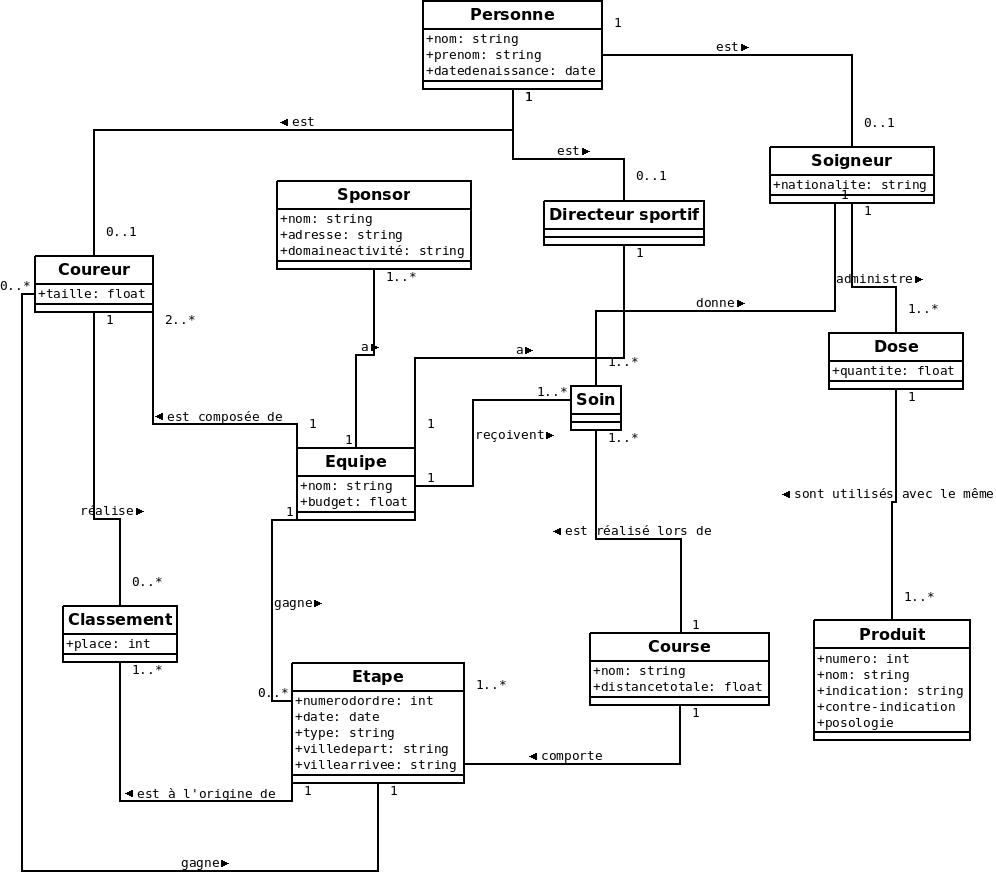
\includegraphics[height=7cm]{img/Figure4.jpg}\\
\caption{Model: Attributes}
\label{fig12}
\end{center}
\end{figure}

This version can be considered as the first version to be proposed to the client based on the initial specifications.
